\documentclass{article}

% Language setting
% Replace `english' with e.g. `spanish' to change the document language
\usepackage[english]{babel}

% Set page size and margins
% Replace `letterpaper' with `a4paper' for UK/EU standard size
\usepackage[letterpaper,top=2cm,bottom=2cm,left=3cm,right=3cm,marginparwidth=1.75cm]{geometry}

% Useful packages
\usepackage{amsmath}
\usepackage{graphicx}
\usepackage[colorlinks=true, allcolors=blue]{hyperref}
\usepackage{subcaption}
\usepackage{listings}

\title{Rust programming language}
\author{Andrea Franceschi}

\begin{document}
\maketitle

\begin{abstract}
This is a personal guide related to Rust programming language from multiple source: Rust.org and papers just included at the end of this guide also the code snipped with light background are taken from "learn rust by example", so take it as it is.
\end{abstract}

\section{Introduction}
\subsection{Types}
\begin{itemize}
    \item i8 / i16 / i32 / i64 / isize
    \item u8 / u16 / u32 / u64 / usize
    \item f32 / f64
    \item bool
    \item char (4-byte unicode)
    \item \textbf{Type inference} for variables \texttt{declarations} with \texttt{let}: so the compiler can infer the type of a variable according to the context and the value assigned.
    \item No overloading for literals: type annotations to disambiguate, operators or functions cannot be overloaded for literals. Cannot define different behaviors for an operator or a function based on the type of literal being used. For instance, you cannot define a different implementation of the + operator to add integers and floating-point numbers.
    \item Tuples
    \item Arrays: with fixed length. Runtime check for out-of-bound!
\end{itemize}

\subsection{Coercion}
Coercion in Rust refers to the \textbf{automatic conversion of one type into another compatible type}. This conversion is performed implicitly by the Rust compiler to make code more convenient and readable.

There are several types of coercion in Rust:

\begin{enumerate}
    \item \textbf{Numeric coercion}: Rust allows implicit conversion between numeric types in certain contexts. For example, you can assign an integer to a floating-point variable without explicitly converting the types.
    \begin{lstlisting}[language=c]
let x: f64 = 5; // Numeric coercion from integer to floating-point
    \end{lstlisting}

    \item \textbf{Reference coercion}: automatically applies reference coercion when passing references to functions or methods. For example, if a function expects a reference to a trait object (\texttt{\&Trait}), you can pass a reference to any type that implements that trait.
    \begin{lstlisting}[language=c]
trait MyTrait {}
struct MyStruct;
impl MyTrait for MyStruct {}

fn foo(x: \&dyn MyTrait) {
    // Function body
}

let my_struct = MyStruct;
foo(\&my_struct); // Reference coercion from MyStruct to \&dyn MyTrait
    \end{lstlisting}

    \item \textbf{Deref coercion}: Rust automatically applies deref coercion when accessing methods or fields on a type that implements the \texttt{Deref} trait. This allows you to treat a reference to a type as if it were the type it points to.
    \begin{lstlisting}[language=c
use std::ops::Deref;
struct MyString(String);
impl Deref for MyString {
    type Target = String;
    fn deref(&self) -> \&Self::Target {
        &self.0
    }
}
fn print_length(s: \&String) {
    println!("Length: {}", s.len());
}
let my_string = MyString(String::from("Hello"));
print_length(\&my_string); // Deref coercion from \&MyString to \&String
    \end{lstlisting}
\end{enumerate}
\\
Coercion in Rust helps reduce boilerplate code and improves the ergonomics of the language by allowing implicit conversions where appropriate. However, it's essential to understand coercion rules to avoid unexpected behavior in your code.




\section{Memory management}

\subsection{ownership}
\begin{itemize}
    \item Each value in Rust has an owner.
    \item There can only be one owner at a time.
    \item When the owner goes out of scope, the value will be dropped.
\end{itemize}
\begin{itemize}
    \item Stack: for activation records
    \item Heap: for dynamic allocated data structures
    \item No implicit boxing: programmer must be aware where data are stored 
    \begin{itemize}
        \item \texttt{let x = 500;} \textit{//x is on the stack}
        \item \texttt{let y = Box::new(500);} \textit{//y is a reference to 500 on the heap}
        \item \texttt{println!("x == y is {}", x == *y);} \texttt{// "x == y is true"}
    \end{itemize}
    \item by the default variables are immutable (cannot change value), can be mutable using \texttt{mut}
    \begin{itemize}
        \item \texttt{let mut z: u8 = 600;}
    \end{itemize}
\subsection{RAII}    
No garbage collector or heap managed by the programmer, Rust uses: \textbf{RAII} Resource Acquisition Is Initialization, \textbf{resources are freed when not needed anymore}, schema: initialization, resource use, destruction
    \begin{itemize}
        \item RAII programming idiom is a software design principle that states that \textbf{resource allocation} occurs during \textbf{object initialization}, through the constructor, while \textbf{resource deallocation} occurs during \textbf{object destruction}, through the destructor.
        \item this means that when an object is created, the necessary resources are acquired and initialized within the object itself, usually in the constructor.
        \item These resources can be memory, files, network connections, or any other resource managed by the operating system or the application.
        \item When the \textit{object is no longer needed} or goes \textbf{out of valid scope} where it was declared, it is automatically \textbf{destroyed}, and the object's destructor is invoked. This \texttt{destructor} is responsible for \texttt{releasing the resources} acquired during the object's initialization. This way, resources are released properly and safely, avoiding memory leaks or resource leaks.
        \item Since \textbf{objects} are \textbf{bound} to the \textbf{scope} (function, block) where they are declared, when the scope closes, objects are destroyed, and any owned resource is released.
        \item \textbf{Each resource has a unique owner}, meaning that the object that acquired the resource is the \textbf{only one responsible for its release}. This ensures that resources are released properly and that there are no resource management conflicts.
        \item \textbf{Ownership can be borrowed as reference} in a mutable or in an immutable manner with lifetime rules (see Figure~\ref{fig:borrow}).
        \item The variable is responsible for managing the lifetime and deallocation of the memory it owns.
        \item \textbf{Borrowing} comes with several restrictions, enforced by \textbf{lifetime} rules. These rules ensure that \textbf{references cannot outlive the data they refer to and that mutable references cannot be aliased}, preventing data races and ensuring memory safety
        \item \textbf{Raw pointers} similar to references, but without the safety guarantees enforced by the ownership system. Operations involving raw pointers that could potentially violate memory safety, such as dereferencing, are marked as unsafe and require explicit handling with the \texttt{unsafe} keyword.
    \end{itemize}
Various mechanisms, including the use of \textbf{traits} (shared behavior across different types), to ensure the RAII (Resource Acquisition Is Initialization) principle. The main traits used to ensure this principle are \texttt{Copy} trait for stack-only data and \texttt{Drop} trait for others.\\If the value has Copy trait, then Rust will duplicate (copy) it in the stack and the older variable is still usable. Otherwise, it will transfer (move) the ownership, thus the older variable is no longer available.
\\These traits determine the way for generating \texttt{lvalue} from \texttt{rvalues} in assignments (left-hand side and right-hand side of an assignment operation), parameter passing, and value returning.
\begin{enumerate}
    \item \textbf{Assignments}: when assigning a value to a variable, the value on the right-hand side (rvalue) is copied or moved to the location of the variable on the left-hand side (lvalue), depending on the behavior defined by the types involved and their traits.
    \begin{itemize}
        \item If the value being assigned implements the \texttt{Copy} trait, it will be copied to the destination location, allowing both the original and the copy to be independently usable.
        \item If the value being assigned does not implement \texttt{Copy} but implements the \texttt{Drop} trait, it will be moved to the destination location. This means that the original variable loses ownership of the value, and it cannot be used afterward.
    \end{itemize}

    \item \textbf{Parameter passing}: Similar to assignments, passing values as function arguments involves moving or copying the values, depending on their types and traits.
    
    \begin{itemize}
        \item If a value is passed by value (not by reference) and it implements \texttt{Copy}, it will be copied to the function's parameter, allowing the function to work with an independent copy of the original value.
        
        \item If a value is passed by value and it does not implement \texttt{Copy} but implements \texttt{Drop}, it will be moved to the function's parameter, transferring ownership to the function and preventing the caller from using the value afterward.
    \end{itemize}

    \item \textbf{Value returning}: When a function returns a value, it can either return the value itself or move it out of the function's scope.
    
    \begin{itemize}
        \item If a function returns a value that implements \texttt{Copy}, it will be copied and returned to the caller, allowing the caller to use the returned value independently of the original.
        
        \item If a function returns a value that does not implement \texttt{Copy} but implements \texttt{Drop}, it will be moved out of the function's scope, transferring ownership to the caller and preventing the function from using the value afterward.
    \end{itemize}
\end{enumerate}
    \begin{itemize}
        \item \textbf{Drop}: for types that require special handling when they are no longer needed. Types implementing the Drop trait have associated destructor logic that is executed when the variable goes out of scope. This allows resources to be automatically released at the end of their valid scope, similar to the RAII (Resource Acquisition Is Initialization) pattern in C++
        \item \textbf{Copy}: for types that can be safely copied by simply duplicating their values on the stack. Types implementing the Copy trait are stack-only data types, and their values are copied when assigned to another variable or passed as function arguments. The older variable remains usable after the copy operation.
    \end{itemize}
\end{itemize}

\begin{figure}[h!]
    \centering
    \begin{subfigure}{0.70\linewidth}
        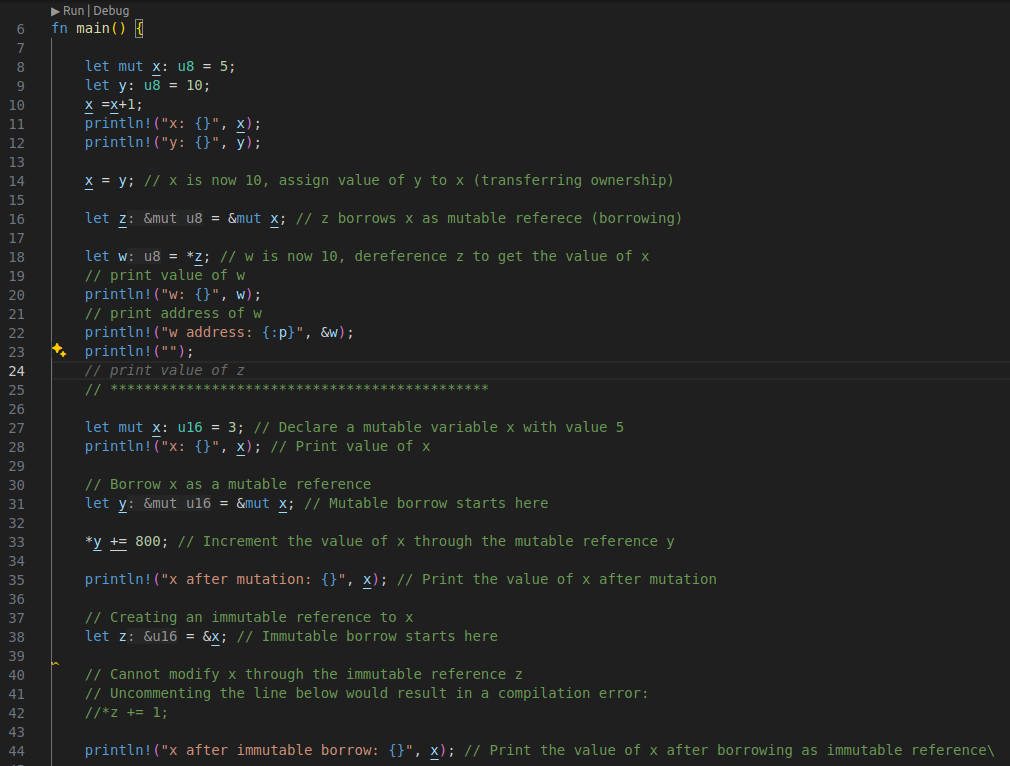
\includegraphics[width=\linewidth]{images/code1.png}
        \caption{code}
        \label{fig:code1}
    \end{subfigure}%
    \begin{subfigure}{0.70\linewidth}
        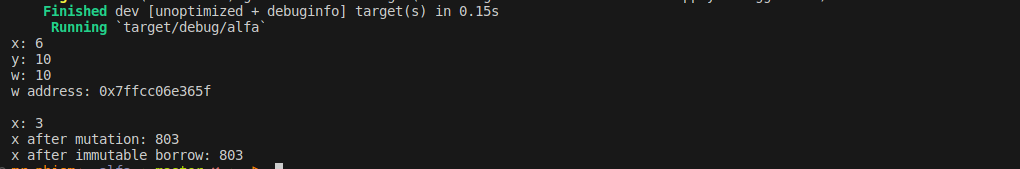
\includegraphics[width=\linewidth]{images/output1.png}
        \caption{output}
        \label{fig:output1}
    \end{subfigure}
    \caption{}
    \label{fig:borrowing_mutable_unmutable_manner}
\end{figure}

\subsection{Ownership}
\textbf{Resource ownership:} \\
In Rust, \textbf{every resource} (such as memory allocated on the heap) is associated with a \textbf{single owner}. This owner is responsible for deallocating the resource when it's no longer needed. Unlike languages with garbage collection, Rust's ownership model ensures deterministic resource management. Note that not all variables own resources (e.g. references).

\textbf{Transfer of Ownership:} \\
When a resource is assigned to another variable (\texttt{let x = y}) or passed as a function argument by value (\texttt{foo(x)}), ownership of the resource is transferred from the previous owner to the new owner. This transfer of ownership is known as a \textbf{move} in Rust terminology.

\textbf{Preventing Dangling Pointers:} \\
Once a resource is moved, the previous owner can no longer access it. This prevents the creation of dangling pointers, which are pointers that reference deallocated memory. By enforcing this rule, Rust guarantees memory safety and eliminates the risk of undefined behavior due to dangling pointers.

\begin{figure}[h]
  \centering
  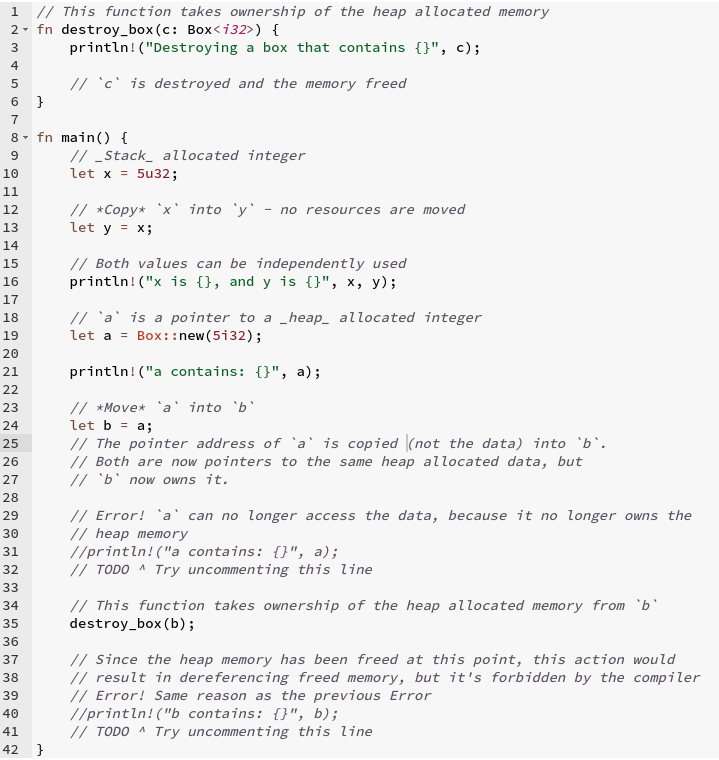
\includegraphics[width=0.7\textwidth]{images/Ownership.png} 
  \caption{This is an example of ownership.}
  \label{fig:ownership_example}
\end{figure}

\subsection{Borrowing}
Rust allow to \textbf{access data without taking ownership} of it. This is where borrowing comes into play. Borrowing allows us \textbf{to pass objects by reference instead of by value}. In Rust, a reference is denoted by \texttt{\&T}, where \texttt{T} is the type of the object being referenced.\\
The borrowing mechanism in Rust ensures memory safety by statically guaranteeing, through its \textbf{borrow checker}, that references always point to valid objects. This means that as long as references to an object exist, the object cannot be destroyed or deallocated. In other words, the compiler ensures that references remain valid and that the referenced data is not modified in unexpected ways.

\begin{figure}[h]
  \centering
  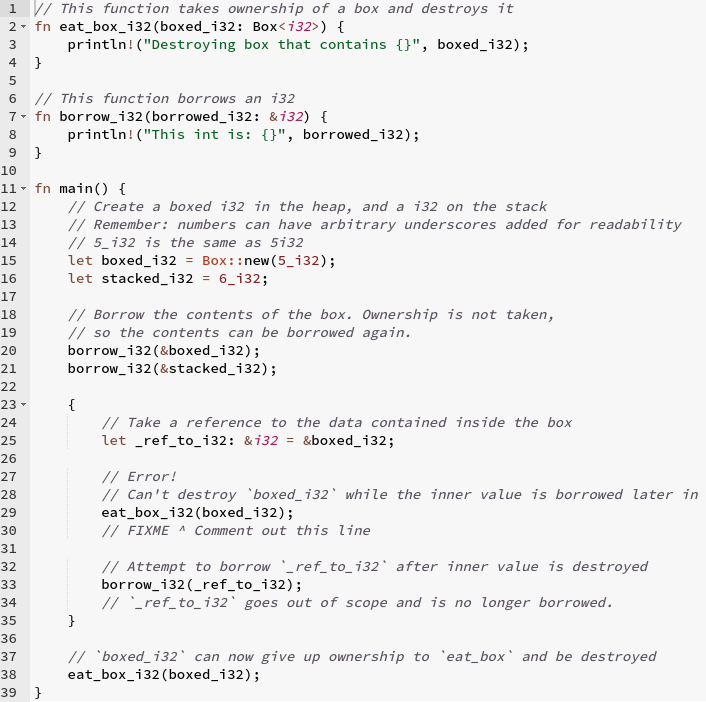
\includegraphics[width=0.5\textwidth]{images/borrowing.png} 
  \caption{This is an example of borrowing.}
  \label{fig:borrowing_example}
\end{figure}
In Rust, \textbf{mutable data} can be \textbf{mutably borrowed} using \texttt{\&mut T}. This is known as a \textbf{mutable reference}, and it provides read/write access to the borrower. With a mutable reference, the borrower can both read and modify the data it references.\\
On the other hand, \texttt{\&T borrows} the data via an \textbf{immutable reference}. With an immutable reference, the \textbf{borrower can read} the data but cannot modify it. Immutable references provide \textbf{read-only} access to the data they reference, ensuring that the data remains unchanged while the reference is active.\\
Can use \texttt{\&'static} to create a reference allocated in read only memory:
\\
\begin{figure}[h]
  \centering
  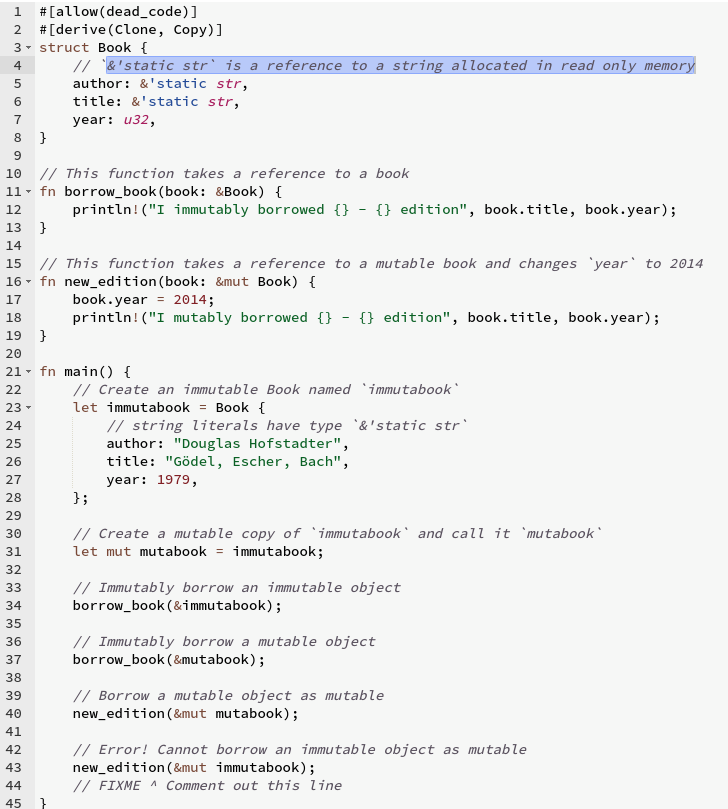
\includegraphics[width=0.5\textwidth]{images/mutable_reference.png} 
  \caption{This is an example of borrowing.}
  \label{fig:mutable_reference_example}
\end{figure}
\\

Can also use the \textbf{ref pattern} where \texttt{ref} borrow on the left side of an assignment is equivalent to an \texttt{\&} on the right side:\\
\texttt{let ref ref\_c1 = c;}\\
\texttt{let ref\_c2 = \&c;}\\
\texttt{println!("ref\_c1 equals ref\_c2: {}", *ref\_c1 == *ref\_c2);}\\
\\


\subsection{Lifetime}
lifetimes are a feature of the type system that ensures references are valid for the duration of their use. Lifetimes specify the scope during which a reference is valid and prevent dangling references or references to deallocated memory.\\
lifetime is a construct the borrow checker's compiler uses to ensure all borrows are valid.\\ Specifically, a \textbf{variable's lifetime begins when it is created and ends when it is destroyed}. While \textbf{lifetimes and scopes are not the same}.
For example, the case where we borrow a variable via \&. The borrow has a lifetime that is determined by where it is declared. As a result, the borrow is valid as long as it ends before the lender is destroyed. However, the scope of the borrow is determined by where the reference is used. A quick summary:

\begin{figure}[h]
  \centering
  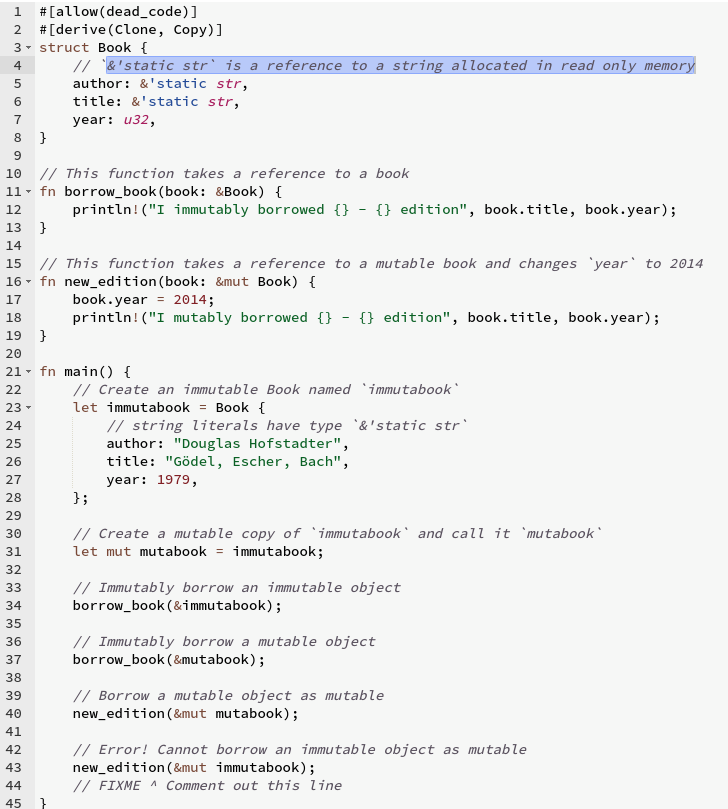
\includegraphics[width=0.5\textwidth]{images/mutable_reference.png} 
  \caption{This is an example of lifetime.}
  \label{fig:lifetime_example}
\end{figure}

\begin{itemize}
    \item \texttt{Scope}: lifetimes are associated with references and indicate the duration for which the referenced data is valid. They are denoted by a tick mark (') followed by a name, such as 'a, 'b, etc.
    \item \texttt{Annotations}: lifetimes can be explicitly annotated in function signatures, struct definitions, and other places where references are used. This helps the compiler verify that references adhere to the specified lifetimes.
    \item \texttt{Lifetime elision}: rules that automatically infer lifetimes in many common situations, reducing the need for explicit annotations. This makes Rust code more concise while still ensuring safety.
    \item \texttt{Borrow checker}: rust's borrow checker analyzes lifetimes to ensure that references are used correctly and safely. It enforces rules such as the borrowing rules, which prevent mutable references from coexisting or overlapping.
    \item \texttt{Parameterized lifetimes}: lifetimes can be parameterized, allowing functions and data structures to work with references of varying durations. This enables generic programming with lifetimes.
    \item \texttt{lifetime bounds}: lifetimes can be bounded to specify relationships between multiple references, such as ensuring that one reference outlives another. This helps prevent dangling references and memory safety issues.
\end{itemize}
\\
\textbf{Explicit annotation}
\\Since the borrow checker ensures memory safety by tracking the lifetimes of references and lifetimes define the scope for which a reference is valid and can be safely used, the borrow checker uses explicit lifetime annotations to determine \textbf{how long references should be valid}.
\\
These explicit annotations specify the \textbf{relationships between the lifetimes of references} in the code. By explicitly defining lifetimes, developers \textbf{can ensure that references do not outlive the data they point to} or are not used after the data has been deallocated, thereby preventing memory safety issues like dangling references or use-after-free errors.
\\
\texttt{foo<'a> // `foo` has a lifetime parameter `'a`}
\\
Using lifetimes requires generics and lifetime syntax indicates that the lifetime of the function \texttt{foo} may not exceed that of \texttt{'a}. Explicit annotation of a type has the form \texttt{\&'a T} where \texttt{'a} has already been introduced.\\
In the following example, the lifetime of \texttt{foo} cannot exceed that of either \texttt{'a} or \texttt{'b}:
\\
\begin{figure}[h]
  \centering
  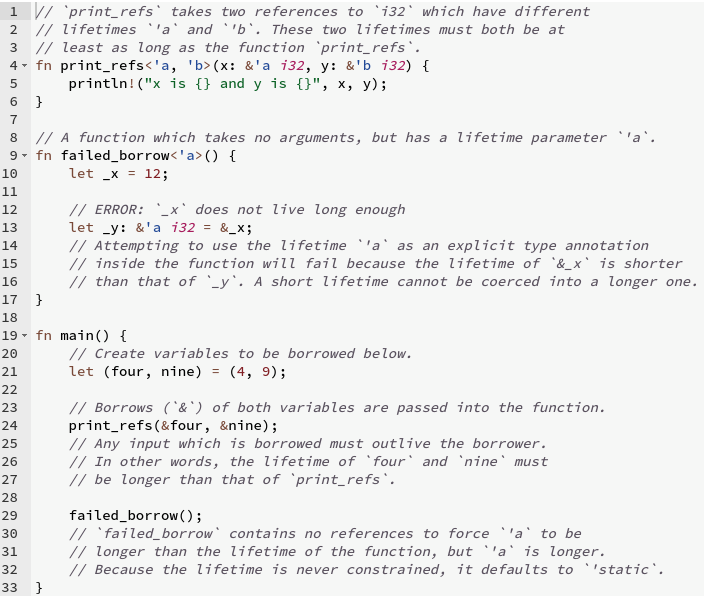
\includegraphics[width=0.5\textwidth]{images/explicit_annotation.png} 
  \caption{This is an example of lifetime.}
  \label{fig:explicit_annotation_example}
\end{figure}
\\
\textbf{Functions signatures with lifetimes} have constraints:
\begin{itemize}
    \item textbf{any reference} used in the function must have an \textbf{annotated lifetime}. This means that when you have references as function parameters or return types, you need to explicitly specify the lifetimes of those references.
    \item If a \textbf{function returns a reference}, that reference must either have the \textbf{same lifetime as} one of the function's \textbf{input references}, or it must be \texttt{'static}. This ensures that the returned reference remains valid for at least as long as the data it refers to exists.
    \item rust prohibits returning references without any input references if doing so would result in returning references to invalid data. This is to prevent the creation of dangling references, which can lead to undefined behavior.
\end{itemize}
Here's an example demonstrating valid function signatures with lifetimes that adhere to these rules (notice that in the function \texttt{fn pass\_x} we can substitute the second input parameter with \texttt{\_: \&'b i32} since is not used inside the function):
\\
\\
\\
\\
\\
\\
\\
\begin{figure}[h]
  \centering
  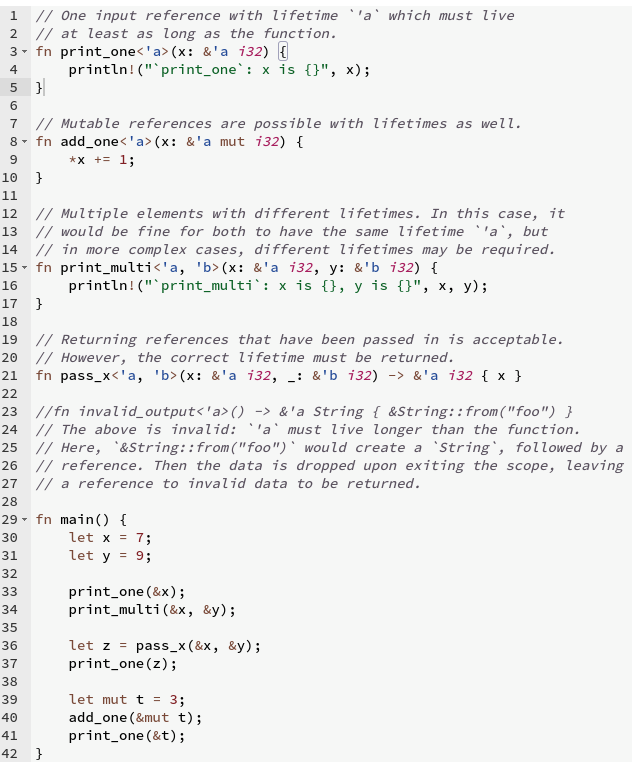
\includegraphics[width=0.5\textwidth]{images/functions_lifetime_annotation.png} 
  \caption{This is an example of lifetime for functions.}
  \label{fig:explicit_annotation_example}
\end{figure}
\\
\textbf{Methods} annotation behave similar to functions:
\\
\begin{figure}[h]
  \centering
  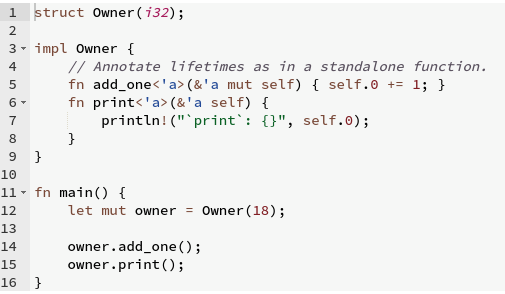
\includegraphics[width=0.5\textwidth]{images/methods_lifetime.png} 
  \caption{This is an example of lifetime for functions.}
  \label{fig:explicit_annotation_example}
\end{figure}

This Rust code defines a structure \texttt{Owner} with a single integer field (\texttt{i32}). Within its implementation, there are two methods:
\begin{itemize}
    \item \texttt{add\_one}: takes a mutable reference to an instance of \texttt{Owner} and increments the value of its integer field by 1.
    \item \texttt{print}: This method takes an immutable reference to an instance of \texttt{Owner} and prints the value of its integer field.
\end{itemize}
In the \texttt{main()} block, an object \texttt{owner} of type \texttt{Owner} is instantiated with an initial value of \texttt{18}. Then, the \texttt{add\_one()} method is called, which increments the integer value within the \texttt{owner} object. Finally, the \texttt{print()} method is called, which prints the updated value of the integer field. The output result will be:
\begin{verbatim}
`print`: 19
\end{verbatim}

\textbf{Struct} annotation behave similar to functions:
\begin{figure}[h]
  \centering
  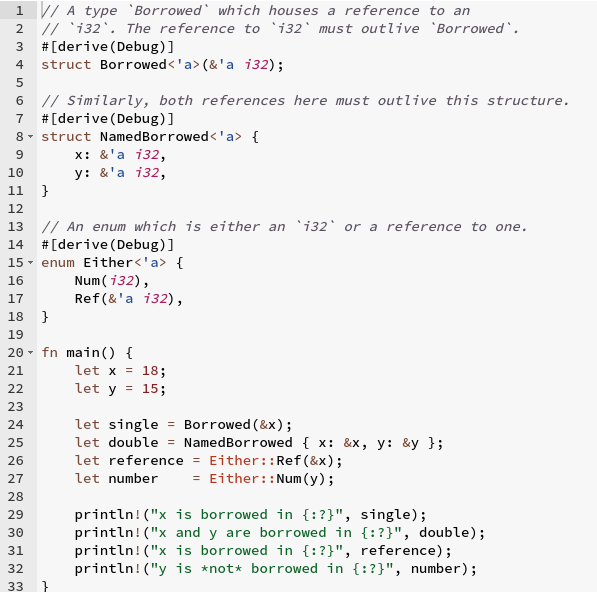
\includegraphics[width=0.5\textwidth]{images/struct_lifetime.png} 
  \caption{This is an example of struct annotation.}
  \label{fig:structu_example}
\end{figure}
\\
This code defines Rust structures and demonstrates borrowing and ownership concepts:

\begin{itemize}
    \item \textbf{Borrowed}: this struct holds a reference to an \texttt{i32}. The lifetime \texttt{'a} indicates that the reference must live at least as long as the struct itself.
    
    \item \textbf{NamedBorrowed}: this struct holds two references to \texttt{i32} values, \texttt{x} and \texttt{y}. Both references must have a lifetime that outlives the struct.
    
    \item \textbf{Either}: this enum can hold either an \texttt{i32} value directly (\texttt{Num}) or a reference to an \texttt{i32} (\texttt{Ref}). The lifetime parameter \texttt{'a} ensures that the reference, if present, must live at least as long as the enum itself.
\end{itemize}

In the \texttt{main()} function:
\begin{itemize}
    \item \texttt{single} is an instance of \texttt{Borrowed}, borrowing the reference of \texttt{x}.
    \item \texttt{double} is an instance of \texttt{NamedBorrowed}, containing references to both \texttt{x} and \texttt{y}.
    \item \texttt{reference} is an instance of \texttt{Either}, holding a reference to \texttt{x}.
    \item \texttt{number} is another instance of \texttt{Either}, containing the value \texttt{y}.
\end{itemize}
\textbf{Traits} annotation behave similar to functions:
\begin{figure}[h]
  \centering
  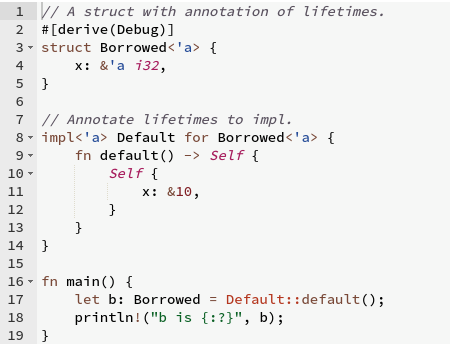
\includegraphics[width=0.4\textwidth]{images/traits_lifetime.png} 
  \caption{This is an example of trait annotation.}
  \label{fig:trait_annotation_example}
\end{figure}
\\
\\
The \texttt{borrowed} struct has a single field x which is a reference to an i32.\\The lifetime \texttt{'a} is used to indicate that the reference may live at least as long as the struct itself.\\
The \texttt{impl} block associates the \texttt{default} trait with the \texttt{borrowed} struct, specifying the same lifetime \texttt{'a} for the default implementation: 
\begin{itemize}
    \item the \texttt{default} method is a convention in Rust for providing a default value for a type
    \item \texttt{default} returns an instance of Self, which refers to \texttt{borrowed}
    \item inside the method body, a new instance of \texttt{borrowed} is created using a struct literal Self { ... }(10-12 lines)
    \item the x field of the \texttt{borrowed} struct is initialized with a reference to the integer 10. This reference has the type \&i32.
\end{itemize}
In the \texttt{main()} function, an instance b of \texttt{borrowed} is created using the \texttt{Default::default()} method, which initializes the x field with a reference to the value 10.
At the end, the value of b is printed.
\\
\textbf{Bounds}: just as generic types can have constraints, lifetimes, which are themselves generic, can also have bounds. These bounds specify relationships between lifetimes and help ensure memory safety.\\
When we see \texttt{T: 'a}, it means that for a type T, all references contained within T must outlive the lifetime 'a. In other words, any reference inside T must remain valid for at least as long as the lifetime 'a.
\\
Similarly, when we see \texttt{T: Trait + 'a}, it means that for type T, it must implement the trait Trait, and all references contained within T must outlive the lifetime 'a. This syntax combines trait bounds with lifetime bounds. It ensures that not only does T implement Trait, but any references inside T also adhere to the lifetime constraint 'a.
\\
\begin{figure}[h]
  \centering
  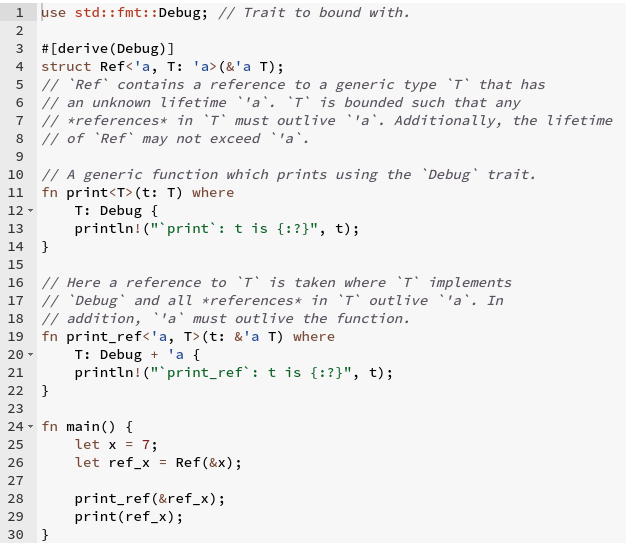
\includegraphics[width=0.5\textwidth]{images/Bounds.png} 
  \caption{This is an example of bounds annotation.}
  \label{fig:bounds_example}
\end{figure}


















\section{Rust compiler}

\subsection{crate}
\textbf{Crate} is a compilation unit, which can be an entire application, a library, or a module within a larger program. Crates are the primary mechanism for organizing code in Rust and provide a form of modularity and code reuse:
\begin{itemize}
    \item Compilation Unit: a crate is a single compilation unit, which can contain one or more modules and their corresponding source code. Each crate is compiled separately into an executable binary file or a library.
    \item Modularity: Crates allow code to be organized into logical modules, making it easier to manage and maintain. Modules can be defined within a crate to separate related functionality and keep the code cleaner and more readable.
    \item Code Reuse: Crates can be used as dependencies in other Rust projects. This allows existing code to be easily reused, encouraging the creation and sharing of open-source libraries.
    \item Dependency Management: Rust uses Cargo, its package and dependency manager, to manage crates and project dependencies. Cargo simplifies dependency management, code compilation, and distribution of Rust applications.
\end{itemize}

\subsection{Invocation}
Compilation starts when a Rust source program is written and \texttt{rustc} invoked, there are some flags es LLVM-IR to extract the LLVM Intermediate Representation  

\subsection{Lexing and parsing}
The raw source code is initially analyzed by a low-level component called a \textbf{lexer}, which is located in a module called \texttt{rustc\_lexer}. The purpose of the lexer is to \texttt{break down the source code} into smaller units known as \texttt{tokens}.\\\texttt{Tokens} are \texttt{atomic units} of source code that represent individual elements such as keywords, identifiers, literals (like numbers and strings), punctuation symbols, and operators. These tokens serve as the \texttt{building blocks} for the subsequent \textbf{stages of compilation}.\\The lexer operates on the raw source text character by character, identifying and \textbf{categorizing each character into appropriate tokens} based on the Rust language \texttt{syntax rules}: in this case lexical-grammar (regular grammar). It recognizes sequences of characters that form keywords, identifiers, literals, punctuation symbols, and operators, among others.
An important feature of the lexer is its support for Unicode character encoding, which allows Rust source code to contain characters from a wide range of languages and scripts.\\After this, the token stream passes through a \textbf{higher-level lexer} located in \texttt{rustc\_parse}. This higher-level lexer prepares the token stream for the next stage of the compilation process.\\At this stage, the \texttt{StringReader struct} is employed to perform a series of \textit{validations} and \textit{to convert strings into interned symbols}. \textbf{String interning} is a technique used \textit{to store only one immutable copy of each unique string value}. This means that if multiple parts of the code contain the same string literal, they will all \textit{share the same underlying memory representation}, reducing memory usage and improving efficiency.
\\The lexer in \texttt{rustc\_parse} has a minimal interface and does not directly rely on the diagnostic infrastructure present in rustc. Instead, it generates diagnostics as plain data, which are later emitted as real diagnostics in \texttt{rustc\_parse::lexer}. This separation allows for a more modular and decoupled design, where the \textbf{lexer can focus solely on its primary task without being burdened by the complexities of diagnostics handling}.\\Furthermore, the lexer ensures that it preserves full fidelity information for both Integrated Development Environments (IDEs) and procedural macros (often referred to as "proc-macros"). This means that the lexer provides detailed information about the structure of the code, allowing IDEs to offer features like syntax highlighting, code completion, and error detection. Similarly, procedural macros, which are used to extend the Rust language with custom syntax, can rely on accurate tokenization provided by the lexer to perform their transformations effectively.\\ Once the token stream generated by the lexer has been produced, it's passed to the \textbf{parser}, which translates it into an \texttt{Abstract Syntax Tree (AST)}. The AST represents the hierarchical structure of the source code in a more abstract and structured form, making it easier for subsequent stages of the compiler to analyze and manipulate and has several properties that aid the further steps of the compilation process:
\begin{itemize}
    \item an AST can be edited and enhanced with information such as properties and annotations for every element it contains. Such editing and annotation is impossible with the source code of a program, since it would imply changing it.
    \item Compared to the source code, an AST does not include inessential punctuation and delimiters (braces, semicolons, parentheses, etc.).
    \item usually contains extra information about the program, due to the consecutive stages of analysis by the compiler. For example, it may store the position of each element in the source code, allowing the compiler to print useful error messages.
    \item ASTs are needed because of the inherent nature of programming languages and their documentation. Languages are often ambiguous by nature. In order to avoid this ambiguity, programming languages are often specified as a texttt{context-free grammar (CFG)}. 
\end{itemize}
The parser employs a \texttt{top-down} parsing, to perform \texttt{syntax analysis}: the parser starts from the top-level constructs of the language grammar and recursively breaks down the input token stream into smaller and smaller parts until it constructs the complete AST.\\
In the Rust compiler codebase, the entry points for the parser are primarily two methods: \\\texttt{Parser::parse \_crate\_mod()} and \texttt{Parser::parse \_mod()}, which are located in the \texttt{rustc\_parse:: parser::Parser module}. \\These methods are responsible for parsing the top-level constructs of a Rust crate or module, respectively.\\For \texttt{parsing external modules}, there's an entry point located in texttt{rustc\_expand::module::parse\_external\_mod}: handles the parsing of Rust modules that are external to the current \texttt{crate} being compiled. Additionally, the parser also serves as the entry point for parsing macros, with the \texttt{Parser::parse\_nonterminal()} method handling the parsing of macro invocations and expansions.
To aid in the parsing process, the parser utilizes a set of utility methods such as bump, check, eat, expect, and look\_ahead. These methods help the parser navigate through the token stream, inspect tokens, and enforce syntax rules defined by the Rust language grammar. Each of these methods plays a specific role in advancing the parsing process and ensuring correctness according to the language specifications.

\subsection{AST lowering}
After the Abstract Syntax Tree (AST) has been constructed, it undergoes a transformation into a \texttt{High-Level Intermediate Representation (HIR)}, which is a more compiler-friendly representation of the AST. This transformation process is commonly referred to as \texttt{lowering}. The AST is transformated and desugared, which involve expanding and formalizing shortened or abbreviated syntax constructs, such as loops and async functions.\\
The \texttt{primary purpose} of lowering the AST into HIR is \textit{to prepare it for subsequent stages of the compilation process}, where more detailed analysis and manipulation are performed. The HIR representation provides a more structured and uniform representation of the code, making it easier for the compiler to perform tasks like type inference, trait solving, and type checking.
\\\textbf{Type inference} is the process of automatically \texttt{determining} the \textbf{types of expressions} in the code without explicit type annotations (i.e.: \texttt{let var = 2;} - we have not defined the type of the variable such that \texttt{let var: u8 = 2}). This is particularly useful in Rust, where the type system is strong but allows for flexibility and conciseness in expressing code.
\\\textbf{Trait solving}: when you use a trait in your code, such as Clone or Display, you're essentially saying, "I want this type to have the behavior defined by this trait." However, traits alone don't provide implementations; they define a set of behavior that types can choose to implement. When the compiler encounters code that uses a trait, needs to find the appropriate implementation of that trait for the specific type being used. \\For example, if you have a function that takes a parameter of type T, and you call a method defined by a trait on that parameter, the compiler needs to find the implementation of that trait for type T.\\
The process of trait solving \texttt{ensures} that the \texttt{compiler can match the trait reference} (e.g., calling a trait method) with the \texttt{correct implementation for the specific type}. This allows for \textbf{polymorphic behavior}, meaning that the \texttt{same code can work with different types} as long as those types implement the required traits.
\\
\textbf{Type checking} is a critical step where the types found in the HIR, representing what the user wrote, are converted into an internal representation used by the compiler. This internal representation, typically denoted as \texttt{Ty<'tcx>}, captures additional semantic information and annotations necessary for further analysis and optimization. Type checking is crucial for verifying the type safety, correctness, and coherence of the types used throughout the program, helping to prevent common errors and ensure robustness in Rust code.

\subsection{MIR Lowering}
the High-Level Intermediate Representation (HIR) undergoes further transformation into the Mid-Level Intermediate Representation (MIR), which is primarily used for \textbf{borrow checking}~\ref{sec:borrow}. Before reaching MIR, the HIR is first converted into THIR (Typed Higher-Level Intermediate Representation), an even more desugared form of HIR, used for pattern and exhaustiveness checking.\\
Once we have the MIR representation, various optimizations are performed on it. MIR is a generic representation, meaning it is not specific to any particular type, which makes it easier to apply optimizations that can improve code generation and compilation speed. Some optimizations are more effective at the MIR level compared to the LLVM-IR level, which is the intermediate representation used by the LLVM compiler backend.\\
One example of an optimization performed at the MIR level is the simplify\_try MIR optimization, which simplifies patterns. While LLVM can perform many optimizations, it may not always recognize certain patterns that can be optimized. By applying optimizations at the MIR level, we can target specific patterns that are more effectively optimized before the code is translated into LLVM-IR.

During code generation, Rust employs a process called monomorphization, which involves generating specialized versions of generic code by replacing type parameters with concrete types. This process ensures that each function or data structure is compiled for every concrete type it is used with, optimizing performance and reducing runtime overhead.

To perform monomorphization, the compiler needs to collect a list of concrete types for which to generate specialized code. This collection process, known as monomorphization collection, occurs at the MIR level. Essentially, the compiler analyzes the MIR representation to identify all the places where generic code is used and determines which concrete types need specialized code generated for them. This ensures that the generated code is efficient and tailored to the specific types used in the program.





\section{Borrow checking}
\label{sec:borrow}








\subsection{How to add Citations and a References List}

You can simply upload a \verb|.bib| file containing your BibTeX entries, created with a tool such as JabRef. You can then cite entries from it, like this: \cite{greenwade93}. Just remember to specify a bibliography style, as well as the filename of the \verb|.bib|. You can find a \href{https://www.overleaf.com/help/97-how-to-include-a-bibliography-using-bibtex}{video tutorial here} to learn more about BibTeX.

If you have an \href{https://www.overleaf.com/user/subscription/plans}{upgraded account}, you can also import your Mendeley or Zotero library directly as a \verb|.bib| file, via the upload menu in the file-tree.

Rust.org

\bibliographystyle{alpha}
\bibliography{sample}

\end{document}